Problem 3: Influence of Hyper-parameters\\
Question 1:\\
\textsl{When we created the T-SNE plot in Problem 1, we ran T-SNE on the top 50 PC's of the data. But we could have easily chosen a different number of PC's to represent the data. Run T-SNE using 10, 50, 100, 250, and 500 PC's, and plot the resulting visualization for each. What do you observe as you increase the number of PC's used?}\\

Answer:\\
With the number of PC's we can influence the explained variance of the data after the reduction of the original data's dimensionality. The more PC's we add to the model, the more accurately we can reconstruct the original data.\footnote{In this case the $log_2(X+1)$-transformed data set from problem 1 was used.} But this does not necessarily mean that, we can get more insight from it.\\ 
	
Therefore we can influence the shape of the T-SNE plot by changing the amount of the PC's (see figure \ref{fig:TSNE_PCs_labelled}). The lower the number of considered PC's, the wider the spread between individual points in one cluster. Besides the density of the data points within one cluster, the distance between individual clusters is affected. With an increasing number of PC's, the clusters start to merge into one another.\\

\begin{figure}[h]
	\centering
	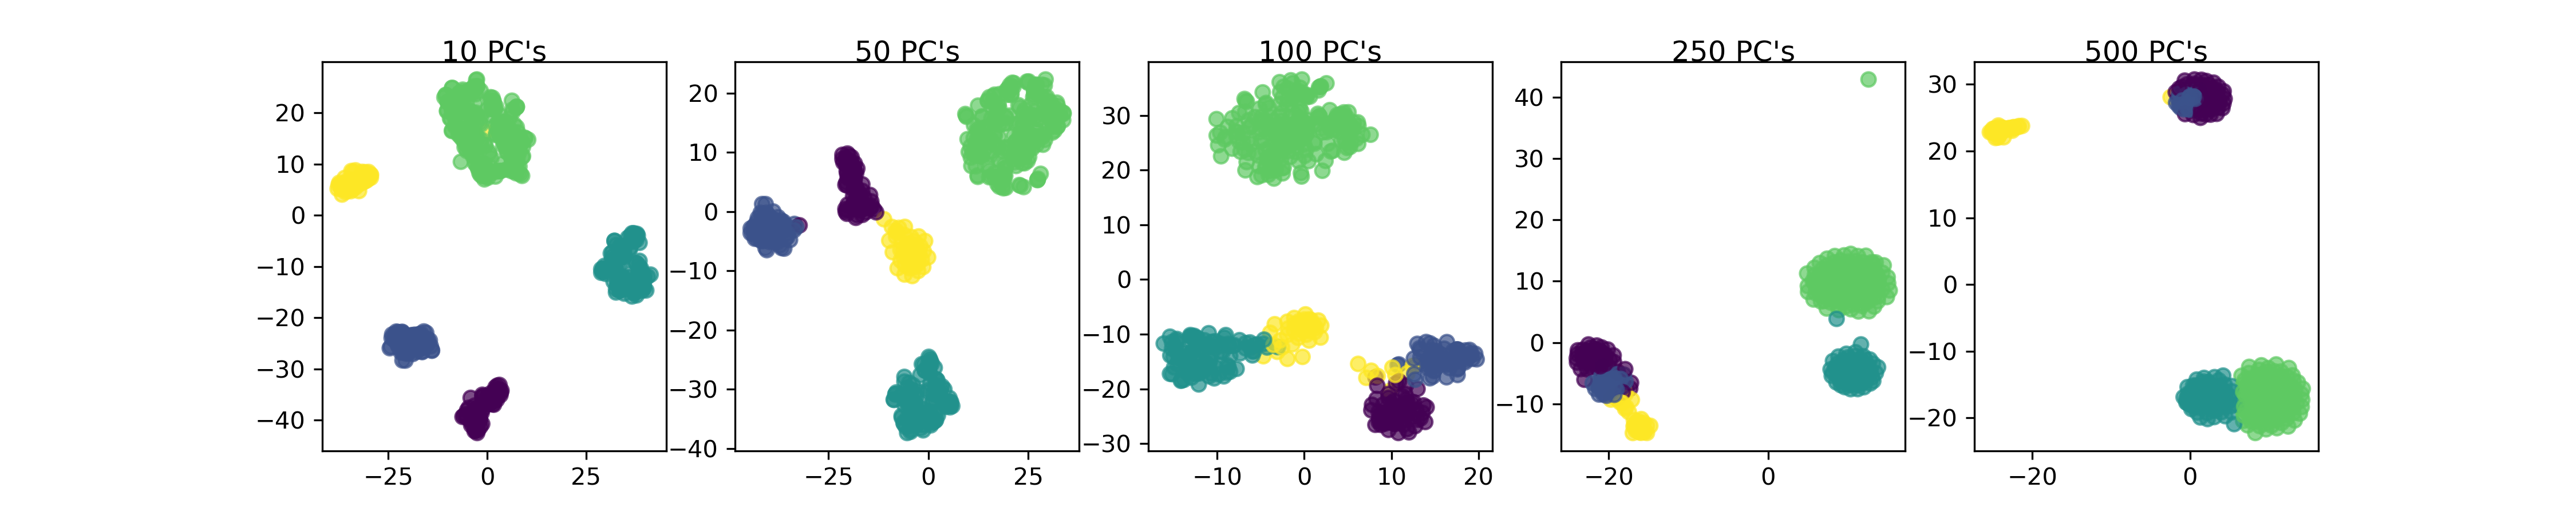
\includegraphics[width=1.0\linewidth, trim={4cm 0 3.5cm 0}]{problem_03/TSNE_PCs_labelled}
	\caption{T-SNE plots for different number of PC's}
	\label{fig:TSNE_PCs_labelled}
\end{figure}

Without knowing the clusters beforehand, we might expect 3 different clusters for 100, 250 or 500 PC's. Therefore, in this example the best visual distinction between the different clusters can be shown by using 10 or at maximum 50 PC's. 